\chapter{Background Research}
\label{chapter2}

% \section{Problem Overview}
% \lipsum[1-1] \cite{parikh1980adaptive}

\section{Virtual Reality}
	Virtual Reality is a technology that has been around since the early 19th century, although in a primitive form through the use of stereoscopic photos \cite{stereoscopy}. Stereoscopic photos work by using two photos that are taken of the same place but are slightly offset from each other, as can be seen in \ref{fig:stereoscope1}. This creates an illusion of depth for the person viewing the images, when viewed through a stereoscope. A stereoscope is a viewing device that only allows one eye to see one of the two images, so each eye sees a similar, yet different image, and this gives the illusion of depth. Stereoscopic vision is the same technology used in current Virtual Reality headsets although now the images are moving.\\


\begin{figure}[H]
	
\includegraphics[width=10cm]{stereoscope}
	\centering
	\caption{Example of a stereoscopic image. \cite{leedsstereoscopic}}
	\label{fig:stereoscope1}
\end{figure}

Virtual reality platforms have been released aiming to provide an immersive experience to consumers. There are many varieties currently available and they can be simply separated in to the two categories: mobile and desktop. Mobile experiences such as the Google Cardboard and Samsung's Gear VR target the audience which already own a compatible mobile device thus eliminating the cost of hardware found in higher end platforms. Through the use of the phone's built in gyroscope and accelerometer, crude head tracking can be achieved to emulate a virtual world.

High end virtual reality platforms target enthusiasts and early adopters of cutting edge technology due to its premium price and high computer hardware requirements in order to run it. Currently there are two virtual reality headsets that are seen as the devices that give highest immersion and these are Facebook's Oculus Rift and HTC's Vive. These will be discussed later in this chapter.

\subsection{Mobile VR}
On the market right now there are two different Mobile Virtual Reality hardware. There is the Samsung Gear VR and the Google Cardboard.

\subsubsection{Google Cardboard}
The Google Cardboard is the cheapest Virtual Reality headset out on the market right now, but it does come with the least features out of them. The cardboard viewer is a stereoscope made out of cardboard. It contains two 40mm focal lenses that are designed to give a distortion when looking through them, which is counter-acted by the distortion from the application\cite{cardboarddev}.
\newline
\par
To use the Google cardboard you would need to install the cardboard application on your compatible phone and then place your phone inside of the Google Cardboard. Once the phone is inside the Cardboard it uses the phone's inertial measurement unit to track head movement. This does have limitations however as the Google Cardboard does not track displacement if the user was to walk in any direction.
\newline
\par
The Google Cardboard still uses the technology of stereoscopic images, as can be seen in \ref{fig:cardboard1}. Although it now does it with moving images, which creates a more immersive experience. \\

\begin{figure}[H]
	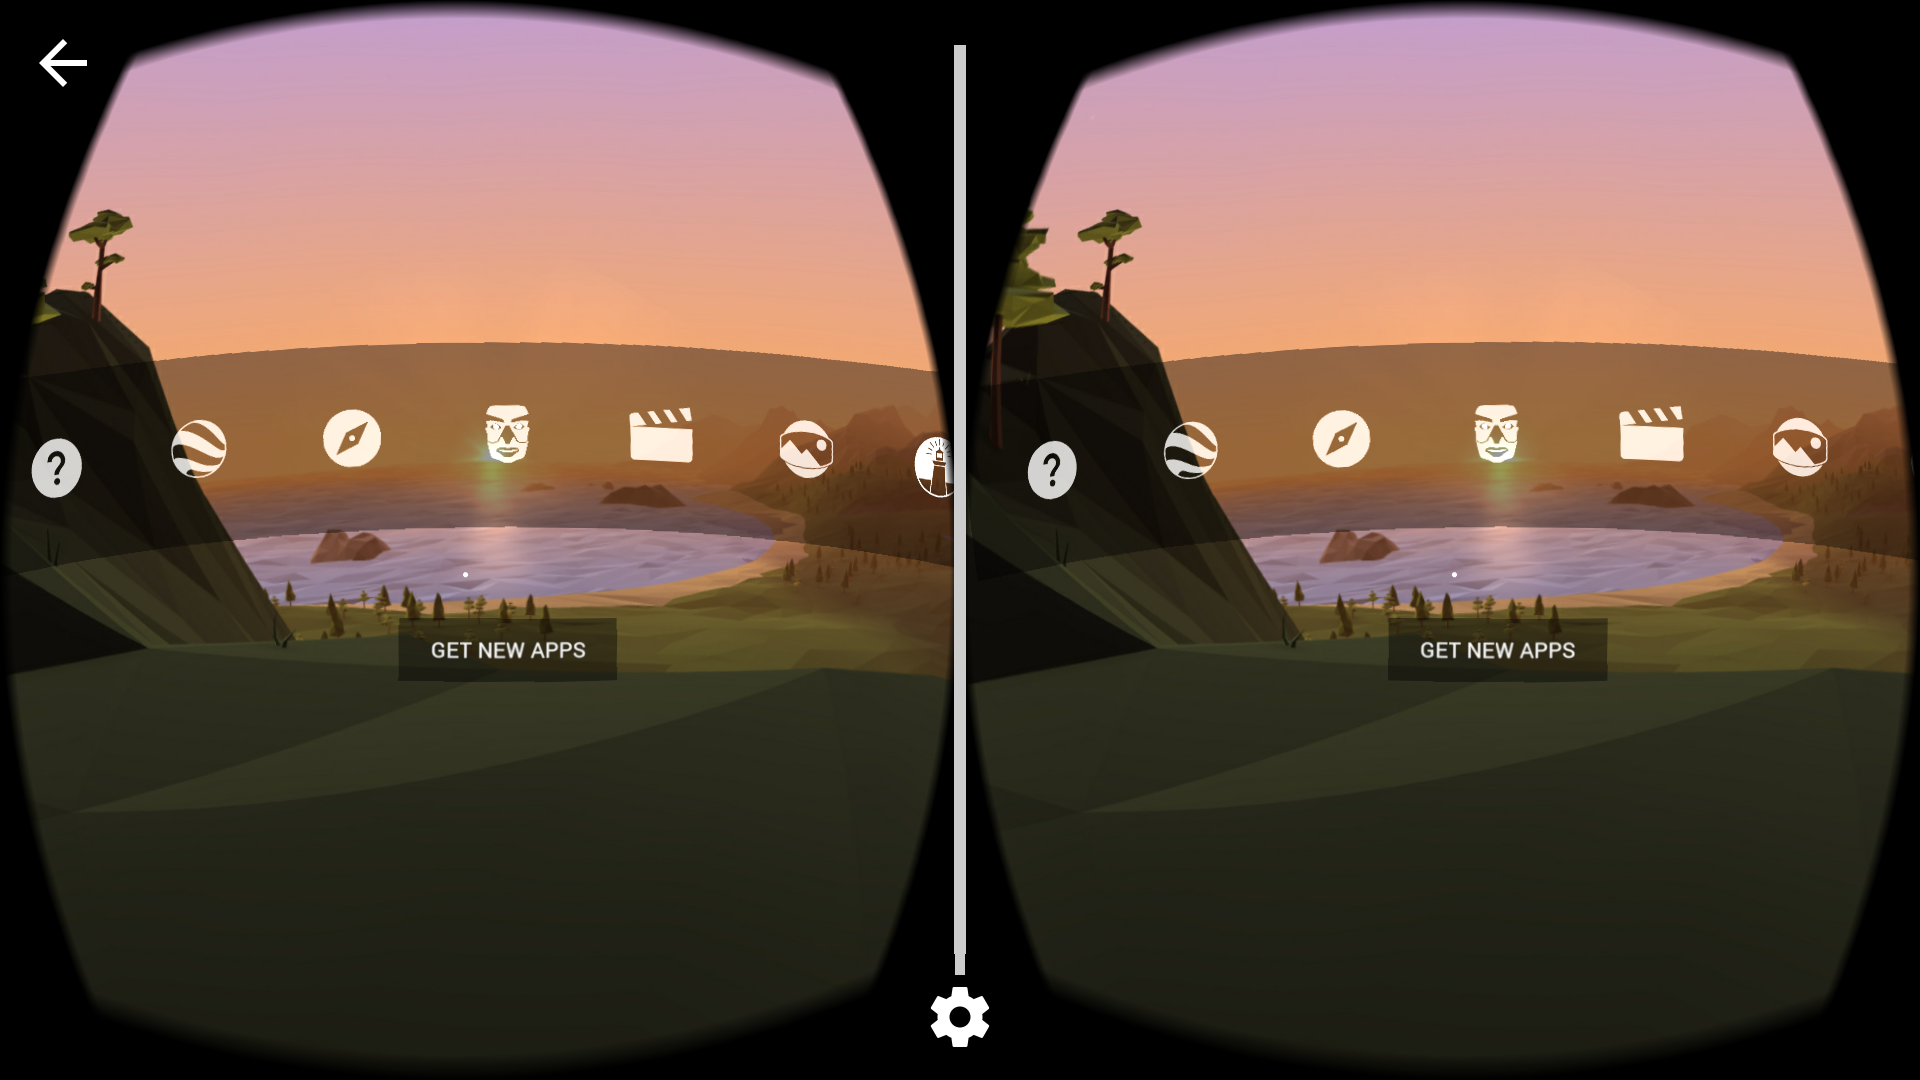
\includegraphics[width=\textwidth]{cardboardscreen}
	\centering
	\caption{Image showing the Cardboard demo application}
	\label{fig:cardboard1}
\end{figure}

The Google Cardboard was not chosen to the virtual reality device for this project as there are many drawbacks to it, and as such it does fully demonstrate all the features present in modern technology for virtual reality. The drawbacks to the Google Cardboard are:

\begin{itemize}
	\item No displacement tracking, making it less immersive than the other options
	\item Only one input method, a button on the cardboard which acts as a screen press.
\end{itemize}

\subsubsection{Samsung Gear VR}
The other mobile Virtual Reality headset on the market is the Samsung Gear VR. The Samsung Gear VR is slightly more expensive than the Google Cardboard, and as expected with the price increase, it comes with more features compared to the Google Cardboard.
\newline
\par
The Samsung Gear VR uses the same technology as the Google Cardboard in the sense that it uses stereoscopic imaging to create the illusion of depth. This is done in the same way for both VR devices, by inserting a compatible phone into the phone holder in the headset, and then showing the stereoscopic images on the phone screen. As seen in \ref{fig:gearscreen} the Samsung gear VR uses the same stereoscopic technology as the Cardboard uses, as seen in \ref{fig:cardboard1}.
\newline
\par
The Samsung Gear VR also uses an inertial measurement unit to detect head movement, similar to the Google Cardboard. The Samsung Gear VR uses an inertial measurement unit contained in the headset, rather than using the attached phone's inertial measurement unit. The inertial measurement unit contained in the headset is more accurate, has lower latency, and is better calibrated than standard phone inertial measurement units, as it uses the same I.M.U. as the Oculus Rift. This I.M.U. is more accurate as it has a higher sample rate than internal phone I.M.U.s and therefore gives it more values to use, so that it can more accurately detect erroneous values.

\begin{figure}[H]
	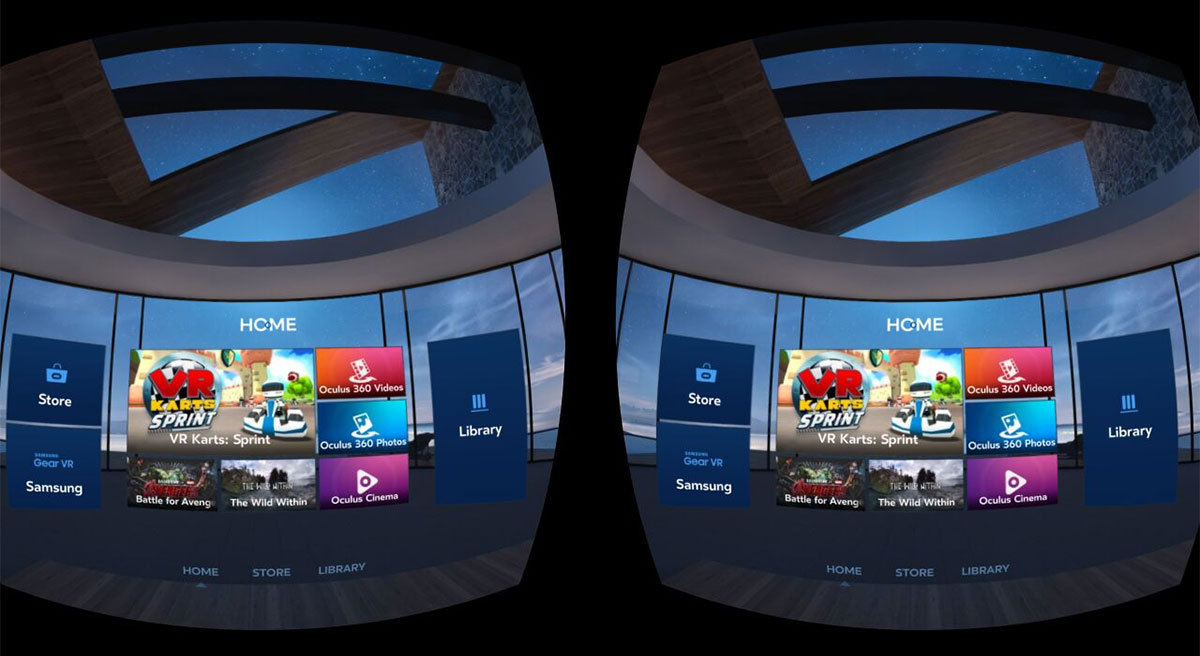
\includegraphics[width=\textwidth]{gearscreen}
	\centering
	\caption{Image showing the Samsung Gear VR menu \cite{gearmenu}}
	\label{fig:gearscreen}
\end{figure}

The Samsung Gear VR has a few extra features compared to the Google Cardboard, for example when a phone is placed inside the Galaxy Gear VR it needs to be connected by a micro-usb connection, which allows the headset to have more input methods to the phone, as well as giving access to the headset's I.M.U. The extra input methods that the Gear VR has access to are:\\

\begin{itemize}
	\item A home button, which works the same as the home button on Android phones.
	\item A back button, which works the same as the back button on Android phones.
	\item A touch pad, which works by swiping to move across menus, and tapping clicks the highlighted item in a menu.
\end{itemize}

\begin{figure}[H]
	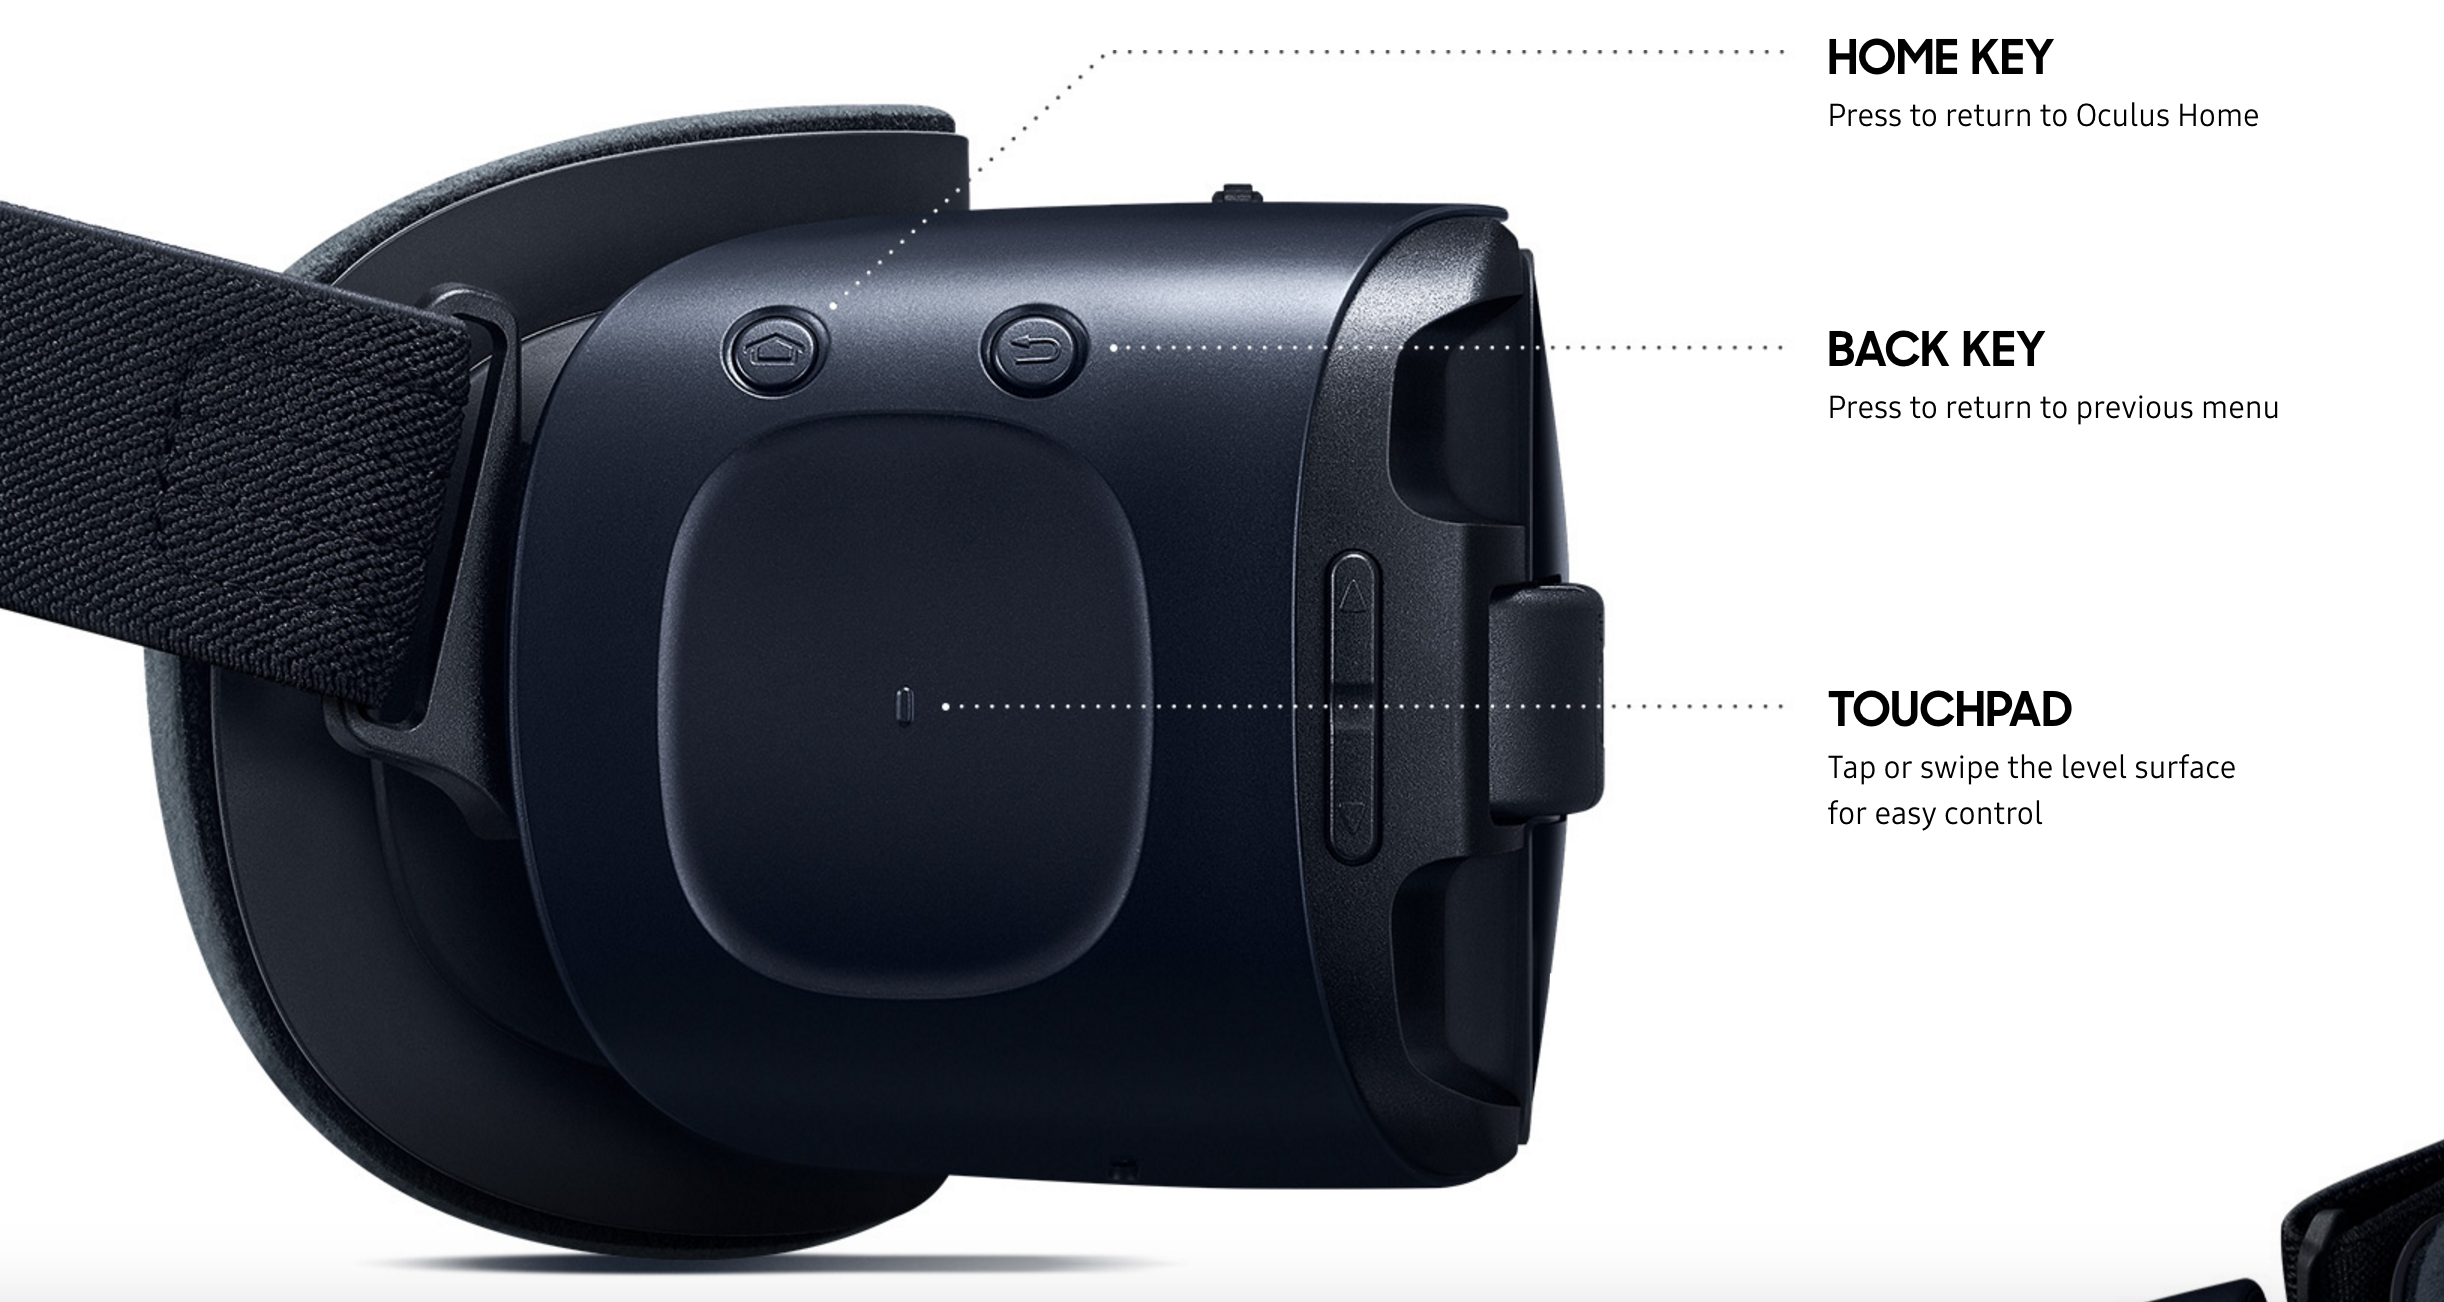
\includegraphics[width=\textwidth]{gearcontrols}
	\centering
	\caption{Image showing the hardware controls on the Samsung Gear VR \cite{gearbuttons}}
	\label{fig:gearcontrols}
\end{figure}

The Samsung Gear VR will not be used for this project as again it has several drawbacks, which are:

\begin{itemize}
	\item It only tracks rotational movement, not displacement, which makes it less immersive than the other options
	\item The Samsung Gear VR has very primitive control, which are only the buttons and touchpad on the side of the headset
\end{itemize}		


\subsection{Oculus Rift}
The Oculus Rift was the first of the two to be released and is inferior in terms of the level of immersion that can be achieved, as currently Oculus only supports interfacing with the virtual world through a third party traditional controller that simply uses buttons and joysticks. The Oculus Rift tracks by using the single camera to pick up infrared light that is emitted by points on the headset. These can be used to track the headset as they blink in a specific pattern, which the sensor knows, and it then uses that to determine the position the headset is in.

\subsection{HTC Vive}
The HTC Vive works using two base-stations. These emit lasers in an alternating pattern, between vertical and horizontal. If these lasers hit a sensor on the headset or controllers, they emit a pulse. By tracking the timings of the laser sweeps and the emitted pulses, the tracking system can use trigonometry to find the position of the location of every sensor on the devices \cite{vivetechnology}. The HTC Vive has two settings, either a sitting or a standing mode. in the sitting mode, it works similar to the oculus Rift, in that a console controller is used to control the game, where as in the standing mode, it uses it's own controllers, which are tracked by the base stations and provide a more immersive experience as you can interact with objects in the game by using these controllers to pick things up by moving your hands to where the object is in game.

% \section{Gaming}
% \lipsum[1-1] \cite{parikh1980adaptive}

\section{Development Environments}
To develop on the HTC Vive there are two options which are currently supported and these are the Unity engine and the Unreal 4 engine. These game engines has native support for SteamVR which is the platform developed by Valve that powers the Vive. Both are free to be installed and just requires a simple registration to their respective websites.
\newline
\par
Unity supports the C\# programming language for development whereas Unreal Engine uses C++ on its current version of the software. Another aspect where it differs is Unity is mainly used to develop games for mobile devices such 2D platformer games. Unreal Engine is mainly used for desktop, AAA games which makes it more suitable for virtual reality with games running on Unreal generally looking better.
\newline
\par
Unreal Engine includes many features built in such as particle effects simulation, terrain, lighting and shading \cite{unrealfeatures}. With SteamVR being natively supported, simple virtual reality features such as gesture recognition and teleportation movement mechanic can be easily implemented in to a game.
\newline
\par
For this project Unreal Engine will be used as the development environment. This is because the group is more comfortable with using C++ so development will be quicker with Unreal rather than trying to use a language with little familiarity.

\subsection{Unreal Engine 4}
The Unreal Engine offers many features for people with little to no programming experience, these will not be used however, as they do not demonstrate any Computer Science expertise, one of the many features that will not be used is the drag and drop interface that is packaged in Unreal Engine to develop simple software quickly, along with the basic templates for various types of games. These are templates for popular genres, for example First Person Shooter and Sidescroller. For this project the group will implement their own features and backend for the genre that is picked, in order to demonstrate their ability to code for the HTC Vive. A select list of the features that Unreal Engine implements already are as follows:

\subsubsection{Unreal Engine 4 Features}
\begin{itemize}

	\item Particle Effects Simulation (Visual Effects)
	\item Procedural Foliage
	\item Landscaping/Terrain
	\item Lighting

	\begin{itemize}
		\item Directional
		\item Point
		\item Spot
		\item Sky
		\item Shadow Casting
	\end{itemize}

	\item Shading
	\item Post Process Effects

	\begin{itemize}
		\item Bloom
		\item Ambient Occlusion
		\item Colour Grading
		\item Depth of Field
		\item Lens Flares
	\end{itemize}

	\item Material Effects
	\item Fog Effects
	\item View Distance Culling
	\item Distance Dependent Level of Detail Models
	\item Physics Simulation
	\item Level Streaming (Ability load and unload map files into memory and toggle their visibility)
	\item Basic Templates

	\begin{itemize}
		\item First-Person
		\item Third Person
		\item Side Scroller
		\item Vehicle
	\end{itemize}

	\item Artificial Intelligence System
	\item Audio System
	\item DirectX 11 \& 12 Features

	\begin{itemize}
		\item Full-scene HDR reflections
		\item Per Scene Dynamic Lights
		\item Physically Based Shading
	\end{itemize}
\end{itemize}

Unreal Engine's full list of features can be found on their documentation site \cite{unrealfeaturelist}
